\documentclass{book}
\usepackage[utf8]{inputenc}
\usepackage{amsmath,amssymb} 
\usepackage{listings}
\usepackage[english]{babel}
%%\usepackage[OT4]{fontenc}
\usepackage{color} % allows to use font color 
\usepackage{url}
\usepackage{graphicx}
\usepackage[bookmarks=true,pdfborder={0,0,0}]{hyperref}
\emergencystretch=11pt
\renewcommand\lstlistingname{Listing}%
\renewcommand\baselinestretch{1.2}
\newcommand{\texttthyp}[1]{\texttt{\hyphenchar\font45\relax #1}}

%%
%%
\makeindex 

%%\bibliographystyle{ddabbrv}
%\nocite{*}

%%
%%
%% ======== METRYCZKA PRACY ========
\title{Development of a WEB Interface for PIPS Compilation Framework}
\author{Maria Szymczak}

\begin{document}
%%\nralbumu{203781}
%%\promotor{Laurent Daverio, Francois Irigoin}
%%\uczelniaNazwa{MINES ParisTech}
%%\uczelniaImienia{}
%%\wydzial{Centre de Recherche en Informatique}
%%\kierunek{Informatique}
%%\specjalnosc{}
%%\specjalnoscdwa{}
%%\rok{2011}
%%\numerRaportu{A/471/CRI}
%%\disclaimer{}

\definecolor{darkgreen}{rgb}{0,0.45,0.08} 
\definecolor{darkgray}{rgb}{0.95,0.95,0.95}
\definecolor{violet}{rgb}{0.5,0,0.33}
\lstset{language=Python}
\lstset{basicstyle=\footnotesize}
\lstset{backgroundcolor=\color{darkgray}}
\lstset{numbers=left, numberstyle=\tiny, stepnumber=1, numbersep=6pt}
\lstset{linewidth=\textwidth, showstringspaces=false}
\lstset{frame=tblr}
\lstset{keywordstyle=\color{violet}\bfseries}
\lstset{commentstyle=\color{darkgreen}}

\maketitle
%%

%%
%%
%% ======== NASZE MAKRA ========
%%

%------------------------------%
\newcommand{\id}[1]{\index{#1}}  
\newcommand{\wi}[1]{#1\index{#1}}  
\newcommand{\wwi}[1]{\emph{#1}\index{#1}}  
\newcommand{\mwi}[1]{\textbf{#1}\index{#1}}
\newcommand{\ii}[1]{\textit{#1}}
\newcommand{\comment}[1]{\textcolor{blue}{\ii{#1}}}
\newcommand{\ourcomment}[1]{\textcolor{red}{\ii{#1}}}
\newcommand{\AWcomment}[1]{\textcolor{red}{\ii{\textbf{#1}}}}
\newcommand{\KPcomment}[1]{\textcolor{blue}{\ii{\textbf{#1}}}}
%\newcommand{}{}
%------------------------------%



%%
%% ======== SPIS TREŚCI ========
%%
\tableofcontents
%%
%% ======== STRESZCZENIE PRACY (POLSKIE) ========
%% \begin{streszczenie}
%%
%% \input{report}
%%
%% \end{streszczenie}
%%

%%
%% ======== GŁÓWNA CZĘŚĆ PRACY ========
%%
%% ==== WSTĘP ====
%%

PaWS is a web interface for the PIPS framework. PIPS is the source-to-source compilation framework (for more detailed information check section \ref{pips_and_pyps}) created by Centre de recherche en informatique of MINES ParisTech \cite{cri}. It is a very complex framework and process its installation is complicated because of many dependencies. With PaWS people can try PIPS without installing it.

With PaWS, user can learn how PIPS works. There are prepared examples which demonstrate PIPS abilities, but users can also try PIPS analyse and transformations on his/her own source code and finally try to change the way how PIPS is working. PaWS provides different levels for different stages of users advance.

PaWS, as it is a web interface, it is a light tool to use, 'thin client', that require no installation but only a bootstraper. Graphical interface is also more intuitive and easy to use for user.

There is also possibility of downloading and setting up user own PaWS instance.

In this document you find a detailed description of PaWS design constraints, design choices, report of the process of creating framework and problems encountered. There is also a technical documentation of the implementation and the configuration of PaWS in section \ref{configuration_guide}. The last section of this document is a user guide.
%% provides information about usage of PaWS.

%% ==== Rozdziały ====

\chapter{PAWS - PIPS as Web Service}

First chapter introduces the idea of creating PaWS framework. It answers the question why it is needed and on what it is based. Design constraints and functional requirements also are presented here. They resulted in emergence of three main modes of using PaWS, which are described in the successive section. Last part of this chapter shows the process of creating the framework.

\section{PaWS}

The introduction page presents overall information about PaWS and PIPS in the panel on the left side, as it is shown in the Figure \ref{fig:intro_page}.

\begin{figure}[h!]
  \centering
  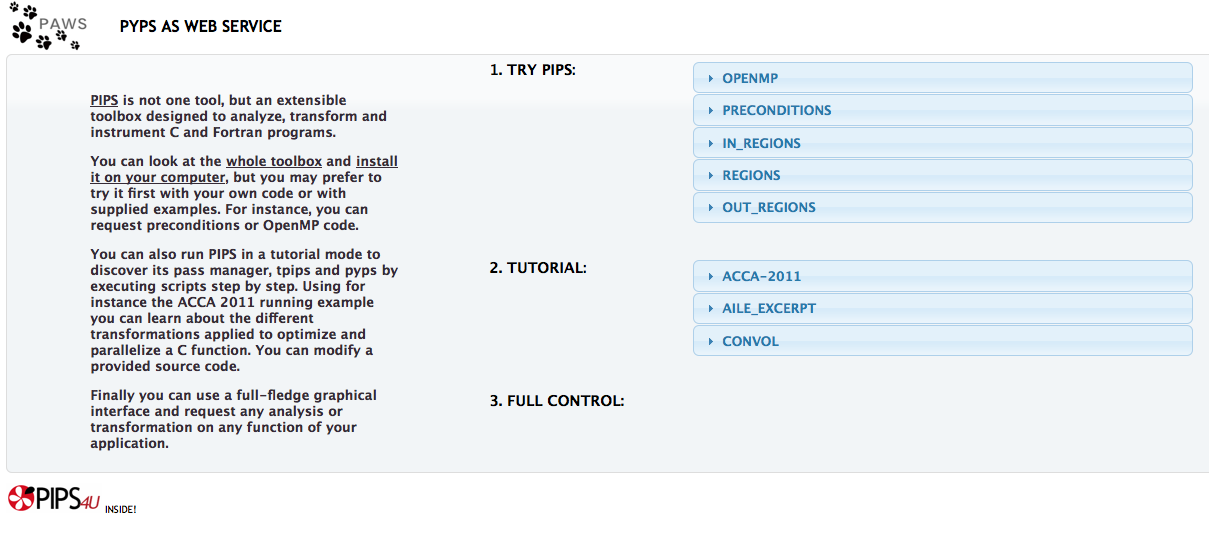
\includegraphics[width=0.8\textwidth]{reportCh4/intro_page}
  \caption{PaWS Introduction page.}
  \label{fig:intro_page}
\end{figure}

Left side panel allows the user to choose mode and its concrete tool or demonstration. To do it, the user has to click on the tab of the chosen tool/demonstration. It will be expanded (see Figure \ref{fig:expanded_tab}) with more detailed information and links to the actual sites visible.

\begin{figure}[h!]
  \centering
  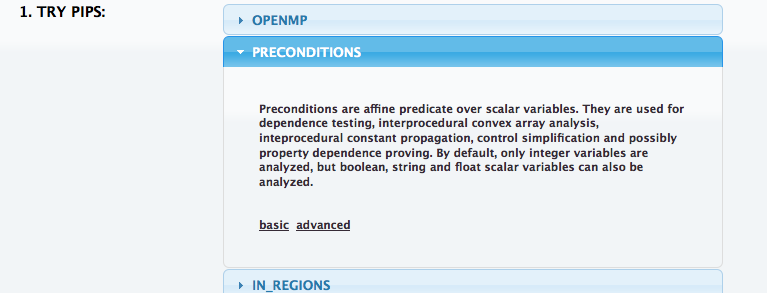
\includegraphics[width=1.0\textwidth]{reportCh4/expanded_tab}
  \caption{Expanded preconditions tab.}
  \label{fig:expanded_tab}
\end{figure}

To come back to the introduction page, the user can use logo image (see Figure \ref{fig:logo_image}) as a link.

\begin{figure}[h!]
  \centering
  
\includegraphics[width=0.2\textwidth]{reportCh4/logo_image}
  \caption{Logo image as home page link.}
  \label{fig:logo_image}
\end{figure}
\section{Design constraints}
\label{design_contraints}

As it is written in the previous section, main goal of the PaWS framework is to create a very light WEB interface for PIPS. It also subjects to other, more detailed constraints:

\begin{enumerate}
  \item {\bf No installation requirements} on a the client side, beyond the browser.
  \item {\bf PIPS scripting complexity is hidden}, result of the operation is ready in few steps.
  \item {\bf Separation of PIPS, PyPS and PaWS} to avoid dependencies between pieces of software and to protect web server from crushing caused by the internal errors.
  \item {\bf Easy customization} of the application for users and developers who are not familiar with PaWS and Pylons. Process of changing particular element is easy, because application is based on the structure of the files which contains python modules with pyps functionalities, examples and files with descriptions of them.
  \item {\bf PIPS server is updated} with recent version of PIPS, wich is propely validated.
  \item {\bf Security} against spamming engines is obtained through the inability to provide Python or shell input.
  \item {\bf Consistency} between:
    \begin{itemize}
      \item the output computed by Tpips and by Pyps;
      \item the output of the cut-and-pasted code, code loaded from the PaWS example, code loaded from the user machine and modified code.
    \end{itemize}
  \item {\bf Using of PIPS validation mechanism}
  \item {\bf Protection against server overload} to assure PaWS availability; control response time.
  \item {\bf Reusability} of existing components as much as possible and generic approach to page creation.
  \item {\bf OS neutrality}
\end{enumerate}

%%  \item {\bf remote execution of PIPS -> demo? not sure}
\section{Design Requirements}
\label{design_requirements}

PaWS framework has several functional requirements, some times related
to the design constraints:

\begin{enumerate}

  \item {\bf Uploading user files (also multiple
      files)}\label{req:uploading_files}: user can provide the source
    code not only by typing or copy-and-pasting it into the
    application window, but also by browsing and picking it from
    his/her machine.

  \item {\bf Saving results on user
      machine}\label{req:saving_results}: user can write back the
    result of the analysis or transformation as a file on his/her
    machine.

  \item {\bf Printing results}\label{req:printing_results}: the user can
    print the result of the analysis or transormation on his/her
    printer.

  \item {\bf Presenting dependence
      graphs}\label{req:dependence_graphs}: user can create and
    display dependence graph of his/her source code. Also
    demonstrations can include graphs.

  \item {\bf Detecting language}\label{req:language_detection}:
    programming language of the source code is detected and
    displayed. C, Fortran77 and, to some extent, Fortran 90 are supported.

  \item {\bf Deleting temporary files}\label{req:deleting_files}:
    temporary files, which are not used anymore, are removed from the
    server disk space.

  \item {\bf Providing ready-to-use examples}\label{req:providing_examples}:
    each analysis and transformation has a set of pedagogical
    examples ready to use by the user.

  \item {\bf Authentication mechanism}\label{req:authentication}:
    access to the PaWS is protected by a simple authentication
    mechanism, a login name and a password.

\end{enumerate}

\section{PaWS Project}
\label{paws_project}

PaWS provides three different modes of using PIPS: tutorial,
elementary analysis or transformation, and full control. Each of them
presents different ways to see how PIPS is working, according to
the user needs.

%% see Introduction for goals
%% implementation vs configuration

\subsection{Tutorial mode}

Tutorial is the PaWS mode that presents PIPS pass managers to users who
are not familiar with this framework. It is also very easy way to
learn how PIPS is working. The user needs only to choose an example
and after it is loaded, he/she can follow transformations and analyses
step-by-step. The user can also skip some steps or go back to previous
ones. There is always a script and its results are presented with some
explanations. The result may include dependence graphs for pedagogical
reasons.

\subsection{Basic analyses and transformations}

This mode enables intermediate users to try specific PIPS
transformations and analysis. The user can choose prepared examples or
use his own code to see how PIPS works. He can later modify the source
code to see differences in results. PIPS related analyses and
transformations are available at two levels: basic and advanced. Basic
level performs operations with default PIPS properties. The advanced
level provides list of properties, that can be modified by the user to
obtain more accurate results or ot speed up PIPS. More information can
be found in the configuration chapter (see Section~\ref{currentconfiguration}).

\subsection{Full control}

Full control is the mode that enables users to create graphically PyPS
or TPIPS scripts which are applied later to the source code.

This mode has not been implemented yet.

\section{PaWS Development Process}

PaWS framework was created with a Agile Methodology
\cite{agilemethodology}. The whole process was made of several short iterations,
each adding new capabilities to PaWS. Each iteration had its
own list of the requirements refering to the general PaWS design
requirements and constraints (see Sections \ref{design_contraints} and
\ref{design_requirements}). After completing an iteration, it was
summed up and, according to its result, the main goals might have been
slightly modified. The list of the encountered problems is given in Section
\ref{encountered_problems}.

The goal of the first iteration was to create working skeleton of the
framework, which was linking Pylons and Pyps technologies together. It
could only perform \emph{preconditions} analysis. The next steps
included the addition of
new PIPS passes and the customization of WEB pages with
user-friendly features such as saving, printing results, and source code
colorization. Further action was to extend PaWS with the second mode -
demonstration and by possibility of creating graphs.

At the same time, consistency and stability of the PaWS framework (see Section \ref{encountered_problems}) has been being improved.

The goal of the last step of the project was to improve the existing
framework by writing tests, scripts for administrators to add new tool
or demo, refactor code and framework structure, and implementing
several user-friendly features such as the uploading of an
archive file. PaWS also was included in the PIPS building process.

%% TO DO: About process of creating PaWS application - from what we started, what was added, what was not good idea.
%% trial and error process
%% no ... agile programming
%% V CYCLE, AGILE

%% exploratory process, agile development, validation, evaluation




\section{Conclusion}

PaWS is a lightweight and easy to use application, although it refers to a very complex toolkit, which is PIPS. Design contraints and requirements which were evolving over the time and also different modes of using this framework with significant amount of examples resulted in necessity of providing flexibility in configuring and changing PaWS. It required using good architectural solution and proven tools or libraries. These issues are described in subsequent chapters.

``Web service'' in the PaWS acronim should not be taken literally. It is not the implementation of the Web Service standard \cite{ws_standard}. PaWS framework idea refers to the conception of the service\footnote{Service is the independent software element which shares complete, reusable  functionality through the well defined interface \cite{service_def}.} in general. The term ``web'' in this case means that functionality shared by the PaWS service is available via the Internet.


\chapter{Implementation}

PaWS is a very light and portable framework. This is achieved by using
multiple flexible and easy-to-extend technologies and tools, that are
presented in this section. All aspects related to the implementation
of PaWS are introduced with an architecture description and an
overview of specific solutions used. The last part of this chapter
contains information about problems encountered during the development
process.

This chapter must be read to understand how PaWS is working. It is
also a great introduction to Chapter 3, namely the configuration of
the PaWS framework.

\section{PaWS architecture}

This section presents the general software architecture. At first, the base and high-leveldescription of the architecture concept is introduced. The next subsection describes elements of PaWS framework and their relations. Scenarios of PaWS operations are also included.

\subsection{\emph{Model-View-Controller} design pattern}
\label{mvc}

\begin{figure}[h!]
  \centering
  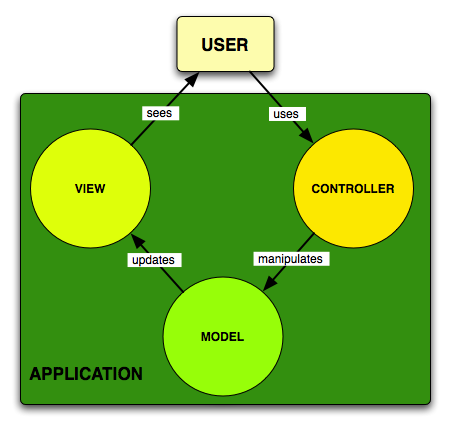
\includegraphics[width=0.5\textwidth]{reportCh2/mvc}
  \caption{MVC concept\cite{mvc_for_php}}
  \label{fig:mvc}
\end{figure}

PaWS is based on MVC\cite{mvc} design pattern. MVC stands for \emph{Model-View-Controller} and is an architectural design pattern for software engineering, especially for creating applications with graphical user interface. 

As can be seen on the figure \ref{fig:mvc}, MVC divides the application into three parts: 
\begin{itemize}
  \item {\bf Model}, which is the representation of problem or application logic, 
  \item {\bf View}, which describes how to display some parts of model in the user interface,
  \item {\bf Controller}, which is responsible for communication with user, like receiving input data or updating model and refreshing view in reaction to user actions.
\end{itemize}

In PaWS framework, the Model layer is not present, because there is no specific data logic and nor database is used. However, PaWS could be extended by adding for example user authentication or customization for users (like remembering preferences) and, in this case, a database (and Model layer) will be necessary.

\subsection{Architecture overview}

PaWS is a framework which shares its functionality remotely. 
\begin{figure}[h!]
  \centering
  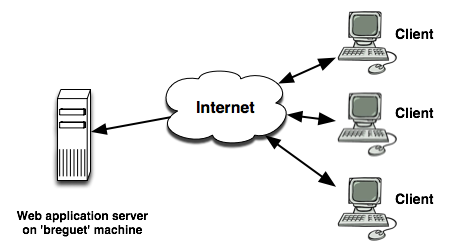
\includegraphics[width=0.5\textwidth]{reportCh2/web_applications}
  \caption{Architecture of access to web applications}
  \label{fig:web_applications}
\end{figure}
That means that there is no need of installing it on the machine of client and PaWS can be reached via the Internet as it is presented in the Figure \ref{fig:web_applications}. Clients need only a web browser - so called \emph{thin client}. A \emph{Thin client} can be a terminal or a computer. It needs another machine (its server) to perform its tasks. Advantages of this approach is lack of necessity to install special tools on client machines, independence from changes of software on the server and low load of the clients machine. Disadvantages of this solution may be: reduced functionality on the client side, requirement to establish internet connection to perform the tasks and all of the limitations resulting from the usage the network (latency, bandwidth).

In addition, in PaWS there is PIPS running, as it is presented on the figure \ref{fig:webapp_paws}. What is more, Pyrops (which is described in section \ref{other_technologies}) enables remote usage of PIPS and what follows, distribution of the application is case of load balancing.


\begin{figure}[h!]
  \centering
  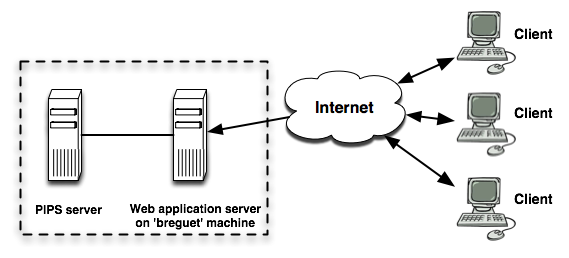
\includegraphics[width=0.5\textwidth]{reportCh2/webapp_paws}
  \caption{Architecture of access to PaWS}
  \label{fig:webapp_paws}
\end{figure}

PaWS architecture is not complicated and consists of 3 layers. It is presented in the Figure \ref{fig:paws_architecture}.

\begin{figure}[h!]
  \centering
  
\includegraphics[width=0.7\textwidth]{reportCh2/paws}
  \caption{Architecture of PaWS}
  \label{fig:paws_architecture}
\end{figure}

The top layer is {\bf PaWS web application}. It consists of:

\begin{itemize}
  \item {\bf HTML code} part, which is responsible for graphical user interface. It is equivalent of the 'View' layer in MVC. HTML sites are built on the basis of the relevant templates in the Mako language. Each PaWS mode (like tutorial, basic tools etc.) has separate templates for creating adequate site. Content of web pages is supplied by structure of files with descriptions (i.e. examples or PIPS basic tools). {\bf Ajax} part of this layer is responsible for the dynamic content of the site and for communication with controllers layer, i.e. for passing variables between those two layers.
  \item {\bf Pylons controllers} part, which is responsible for interception and interpretation of the user input. It also can pass output back to the view layer. Pylons controllers are a simple and powerful solution. They are special Python classes, which are very easy to customize. In PaWS, the controllers layer is also responsible for passing input and getting output of operations of lower layers.
\end{itemize}

The two lower layers are linked together very tightly. The middle layer is composed of three parts. The first of them, {\bf Pylons} is the core of web application and provides all web server functionalities described in section \ref{pylons_descriptions}. The other two parts: PyPS (see: \ref{pips_and_pyps}) and Tpips (see: \ref{tpips_interface}) are interfaces for PIPS framework.

The lowest layer is the kernel of the whole system and is composed of two parts:

\begin{itemize}
  \item {\bf Python} (described in \ref{python_description}), which is the base for Pylons and PyPS mechanisms.
  \item {\bf PIPS core} (described in \ref{pips_and_pyps}), which provides all of the transformations and analysis.
\end{itemize}

Middle layer with interfaces is necessary for proper activity of PaWS. Both Tpips and PyPS simplifies usage of PIPS and encapsulate its functionalities. What is more, due to PyPS it is easier to link Pylons Controllers with PIPS operations - it enables to invoke PIPS methods from Python code (directly in controller or by importing prepared modules).

\subsection{Structure}
\label{structure}

PaWS framework files and directories structure consists of two main parts: Pylons related and PIPS related.

\begin{figure}[h!]
  \centering
  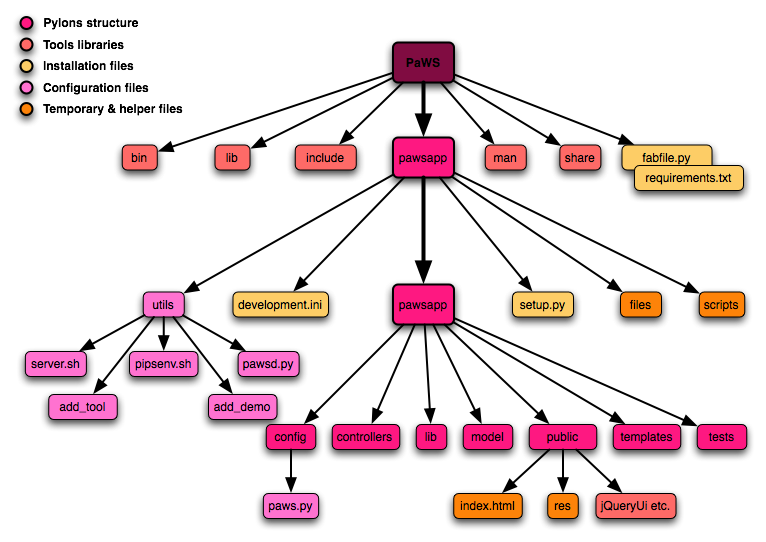
\includegraphics[width=1.0\textwidth]{reportCh2/paws-structure}
  \caption{File structure of PaWS}
  \label{fig:paws_structure}
\end{figure} 

The first one, shown in the Figure \ref{fig:paws_structure}, is based on Pylons project directories structure. Files and directories here can be classified into 5 types:
\begin{enumerate}
  \item {\bf The Pylons structure} directories which contain source code of PaWS framework. They are described in following section \ref{architecture_elements}.
  \item {\bf The installation files} - files used during the process of installation PaWS on user's machine. Two of them \emph{development.ini} and \emph{setup.py} refer to Pylons directly and can be also used as a configuration files. \emph{Fabfile.py} and \emph{requirements.txt} are the files of Fabric framework (see section \ref{other_technologies}) designed for quick installation of the all dependencies of PaWS framework. More details can be found in the section about PaWS installation \ref{installation}.
  \item {\bf The configuration files} - all of the files which can be modified by user to get the proper settings for his PaWS instance. To this group also scripts to manipulate the application content are belonging:
  \begin{itemize}
    \item {\bf add\_tool}: a script used to add a new analysis or transformation, described in the Section \ref{add_analysis_transformation}.
    \item {\bf add\_demo}: a script used to add a new demonstration, described in the section \ref{add_demonstration}.
    \item {\bf pipsenv.sh}: a script which is responsible for adding necessary directories to the path and system variables.
    \item {\bf pawsd.py}: a script which is responsible for deleting old temporary files.
    \item {\bf server.sh}: a script for starting application server.
  \end{itemize}
  \item {\bf Temporary and helper files} created by PaWS - directories and files which are necessary for PaWS work, but are not the part of Pylons architecure. They should not be changed by a user. Directories \emph{files} and \emph{res} are storing files temporary created during the PIPS operations, directory \emph{scripts} containts scripts related to adding new functionalities of PaWS and \emph{index.html} is responsible for redirectoring user to the PaWS introduction web page.
  \item {\bf Libraries} - directories and files of the tools which support work of PaWS, like VirtualEnv (described in \ref{virtualenv}) section or web applications technologies libraries (described in \ref{web_application_technologies} section).
\end{enumerate}

On the highest level there are mainly libraries and binaries related to the tools used by PaWS, i.e. Virtualenv described in \ref{virtualenv}.

The second part of PaWS structure used for configuration, presented in the Figure \ref{fig:pips_structure}, is located in the PIPS \emph{validation} directory and is mapping abstract PaWS division into modes, such as tutorial or full control (described in section \ref{paws_project}) onto the physical directories structure.

\begin{figure}[h!]
  \centering
  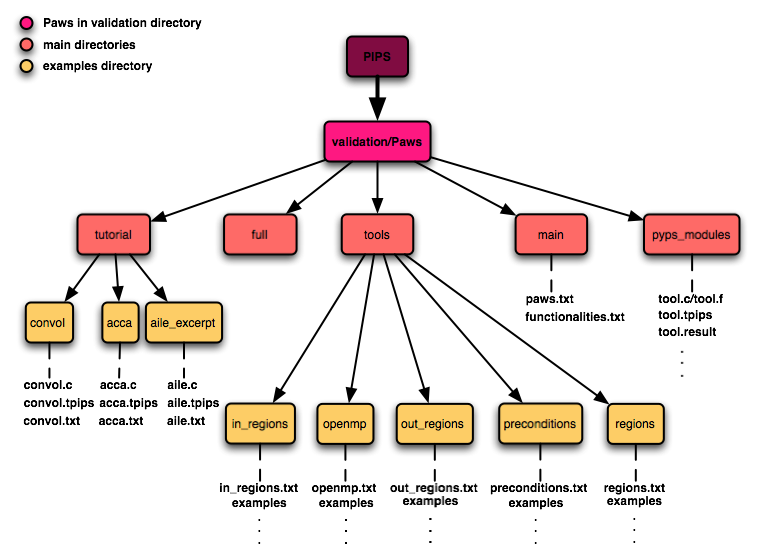
\includegraphics[width=1.0\textwidth]{reportCh2/pips-structure}
  \caption{Structure of PIPS part of PaWS}
  \label{fig:pips_structure}
\end{figure}

\subsection{Architecture elements}
\label{architecture_elements}

This section contains descriptions of the main types of PaWS framework elements: controllers, templates, validation directory and libraries.

\subsubsection{Controllers}

As it is described in the previous section, controllers are responsible for performing actions at the user request. In PaWS several types of controllers are used. 

\begin{enumerate}
  \item Controllers responsible for hosting web sites and contains only one method ``index''. They are created automatically when adding new functionality. Their names correspond to the functionality they respresent (i.e. ``tools preconditions'' or ``tutorial convol'')
  \item Controllers responsible for creating special web sites, like ``paas'' controller for introduction page or ``descriptions'' controller for extracting information from the structure of description files.
  \item Controllers responsible for linkage with PyPS or Tpips for performing operations. There are three controllers this type: ``operations'' for basic tools (both basic and advanced level), ``demo'' for tutorial and ``graph'' for creating dependence graps.
  \item Controllers for other operations which are not using PIPS. To this group belong controller ``detector'' responsible for detecting language of source code and ``examples'' controller which is loading supplied examples.
\end{enumerate}

\subsubsection{Templates}

Templates are the files which provide code for web sites. They are a very convenient solution because they allow to combine HTML, Javascript and Python code. What is more, especially when web application consists of many similar pages, templates technology allows to use the inheritance between templates. That significantly reduces the amount of redundant code. 

PaWS consist of several types of templates:

\begin{itemize}
  \item ``Skeleton'' templates, which provide necessary (and common for all of the pages) operations for application to work (like uploading files, changing font size or checking if the input source code is correct). Those templates (like ``frame'' template) are creating structures which are inherited by other, more specific, templates.
  \item Templates which are creating frame code dedicated to the specific PaWS mode (like tutorial, basic PIPS tools or advanced PIPS tools). They are inheriting from more general skeleton templates. 
  \item Templates which are responsible for creating specific web site dedicated to the special case (one tutorial or PIPS tool). Each of them inherits from the appropriate mode template and provides characteristic information, such as the name of the PIPS tool or the name of tutorial file.
  \item ``Paas'' template which is responsible for introduction page, and for extracting information about available tools from the description files.
\end{itemize}

\subsubsection{Other modules}
\label{other_modules}

PaWS consists also of some other modules:

\begin{itemize}
  \item {\bf \emph{validation}} is the directory of PIPS project where all the supplied examples are placed. All of the samples each day undergo validation. PaWS validation directory is placed in PIPS repository in \emph{validation/Paws} and consists of several directories:
  \begin{itemize}
    \item {\bf \emph{pyps\_modules}} described below;
    \item {\bf \emph{tutorial}} which contains all of the demonstration examples;
    \item {\bf \emph{tools}} which contains subdirectories with examples dedicated to concrete tool (like \emph{preconditions} or \emph{openmp}). Those directories are named after mode they refer to;
  \end{itemize}
  \item {\bf PyPS modules} are the part of \emph{validation} directory (named \emph{pyps\_modules}). Each module contains PyPS code necessary to perform some analysis or transformation. As all of the cases kept in \emph{validation} directory because those modules also should undergo validation each day.
  \item {\bf \emph{public}} is the Pylons directory where all of the helper but not directly connected to the Pylons or PIPS tools and features are placed. In example, all of the Javascript libraries, images used by PaWS or description files are stored here. 
  \item {\bf \emph{lib}} is the Pylons directory for all of the helper Python libraries and modules used by PaWS (like base Pylons controller, helper for managing files or detectors of programming languages).
  \item {\bf \emph{tests}} is the Pylons directory for functional tests for controllers.
\end{itemize}

\subsection{Flows and scenarios}

This section shows how different elements of PaWS architecture are linked together. Basic flows for each mode are presented and described here. Each mode has several cases, different tools or different demo examples, but in each case the scenario of operation performed remains the same.

\begin{figure}[h!]
  \centering
  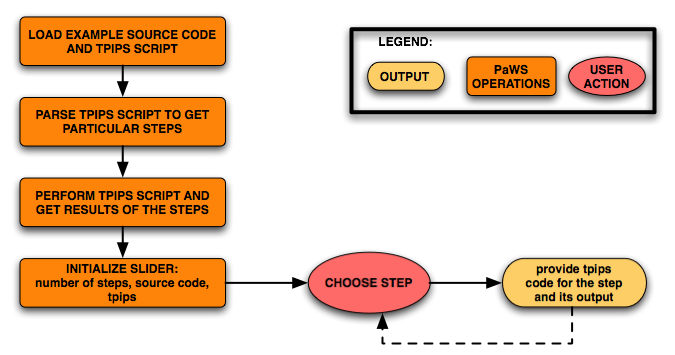
\includegraphics[width=0.7\textwidth]{reportCh2/tutorial_flow}
  \caption{Tutorial flow mode}
  \label{fig:tutorial_flow}
\end{figure}

\begin{itemize}
  \item {\bf Demo mode}: there are three scenarios available: \emph{aile\_excerpt}, \emph{convol} and \emph{acca-2011}. Input and all of the possible operations and their sequence are provided by the application - user only controls the step. The basic flow is presented on the Picture \ref{fig:tutorial_flow}.
  
  \begin{figure}[h!]
  \centering
  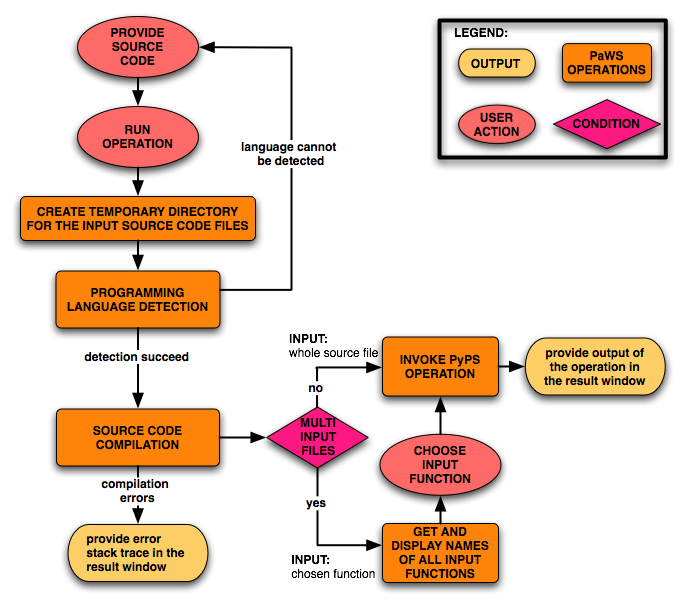
\includegraphics[width=0.7\textwidth]{reportCh2/basic_tool_flow}
  \caption{Basic tool flow mode}
  \label{fig:basic_tool_flow}
\end{figure}

\begin{figure}[h!]
  \centering
  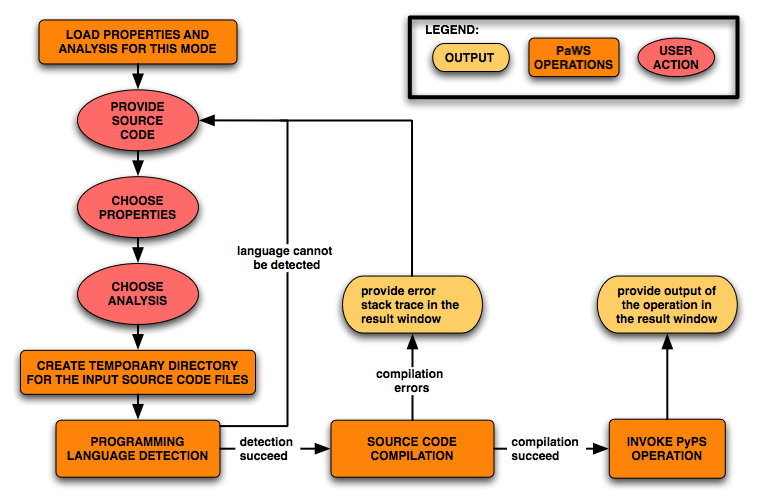
\includegraphics[width=0.7\textwidth]{reportCh2/advanced_tool_flow}
  \caption{Advanced tool flow}
  \label{fig:advanced_tool_flow}
\end{figure}
  
  \item {\bf Basic tools - basic level}: five tools are currently configured: \emph{preconditions}, \emph{IN regions}, \emph{OUT regions}, \emph{regions} and \emph{OpenMP}. This PaWS mode allows user to either choose one of supplied examples, different for each type of tools, or to provide input source code by him/herself (by uploading file or by directly typing or cut-and-pasting in application window). The basic flow of this mode is shown in the Picture \ref{fig:basic_tool_flow}.

  \item {\bf Basic tools - advanced level}: there are two tools available: \emph{preconditions} and \emph{regions}. This mode is similar to the basic level - source code can be provided in the same way here. Basic scenario is displayed on the picture \ref{fig:advanced_tool_flow}.
  
  \item {\bf Full control}: NOT DEVELOPED
  There was not enough time.
\end{itemize}
\section{Selection of the optimal architectonic solution}

The selection of the optimal architectonic solution and libraries used to create the framework is not an easy task. Constraints imposed on the PaWS framework (see Section \ref{design_contraints}) require creation of the web application. It can be done with various programming languages and libraries. 

\subsubsection{Language selection}

One group of languages used in bigger development projects are Java, C++ and C\#. Using them requires program compilation and creation of binary files. Also the programming process requires more programming work and it is not efficient. What is more, C\# is dedicated to the Microsoft Windows operation system which disqualifies its use (see Design Contraints Section \ref{design_contraints}).

The second group of possible languages are scripting languages like Perl, Python, Ruby and PHP. Perl is an obsolete language, but all of them are popular as a languages for web application creation, being constantly developed, free upward-compatible and with lively community, rich documentation, libraries and support. That explains their popularity.

\subsubsection{WEB support}

There are three aproaches to create web application using scripting languages. The first of them is based on CGI\cite{cgi} - Common Gateway Interface. This technology enables communication between web server software and and other programs located on the server. The main disadvantage of this approach is that CGI usually requires the creation a new process for each request. This is not scalable, makes not possible to use the same context and global variables for several requests and can cause server load over very quickly. What is more, CGI does not provide session mechanisms and the Ajax library is not built in.

The second possibility is to use template engines like Cheetah \cite{cheetah} or Jinja2 \cite{jinja2}. The problem is that this solution is too lightweight - it supports only code generation and not provides other useful mechanisms such as routing, session variables handling etc.

The third approach is the most popular approach. It is based on the Model-View-Controller design pattern (described in Section \ref{mvc}). This paradigm supports reusability, separation of layers of the application, is lightweight but easy to extend and takes care of persistent storage if it is needed. There are a lot of framework using the MVC pattern like Pylons \cite{pylons}, Django \cite{django} and Turbogears \cite{turbogears} in Python, Ruby on Rails \cite{rubyonrails} in Ruby and Symfony \cite{symfony}, CakePHP \cite{cakephp} and Yii \cite{yii} in PHP.

\subsubsection{WEB frameworks}

PHP frameworks are more heavyweight and harder to learn than Python and Ruby ones. The most popular PHP web framework - Symphony also has problems with compatibility between its versions which makes difficult to use its support.

Ruby on Rails is a very good framework, but has less support than Pythonic frameworks, because Ruby is younger language than Python. Also Ruby frameworks have performance problems.

The use of Python tools has also other advantages. The main one is the availability of a Python binding in PIPS framework - PyPS, which can be use to dynamically perform PIPS operations instead of creating Tpips (see Section \ref{tpips_interface}) scripts on-the-fly. The selection of Python enables using PyPS in easy way (by importing it as a Python module) but also does not exclude usage of Tpips.

Three Python web frameworks were taken into consideration: Pylons, Django and Turbogears. The last one was rejected because of stability problems\footnote{TurboGears is based on CherryPy \cite{cherrypy} unstable server.}. Despite the fact that Django is more popular than Pylons, the second one was chosen due to greater flexibility. Pylons can be extended with any component the user needs, while Django has a set of its own preferred components. A good example of this problem is the usage of ORM (Object-relational mapping\cite{orm}). Django does not allow to use all of the available toolkits, like the most popular one - SQLAlchemy\cite{sqlalchemy}.

Choosing the Pylons tool and its approach to architecture and structure of the application paid off very quickly - after less than seven days of work, the first prototype of the application was ready and able to communicate with PIPS. 
%% Very significant fact is that PaWS is not the first CRI project based on Pylons and I could count on strong support from more experienced developers.


\section{Technologies used}

This section presents an overview of the key technologies used and their place in the PaWS framework: Tpips, Python, Pylons, Virtual Environment and Web application technologies (Javascript, Ajax and JQuery)

\subsection{Tpips}
\label{tpips_interface}
\emph{Tpips} is the line interface and scripting language of the PIPS project. It allows to use all of the PIPS functionalities in easier (more user-friendly) way, because it simplifies usage of database when performing operations, it handles all accesses to database, for instance itself.
Due to using PIPS metavariables (like \%ALL) Tpips enables application of PIPS command to several modules with one command. Another advantage of this interface is the fact that it provides on-line help (list of commands and automatic completion).
Tpips is a great tool for all tasks which are repeatable and do not require any interaction with the user.

In the PAWS project the Tpips interface is used to perform demo. On source file, even if it was modified by user, there is Tpips script performed with prepared, always the same set of well-known operations. That allows to separate the indivudual steps and their results which are shown to user one by one. Also Tpips script may be more understandable for new user than PYPS code.

\subsection{Python}
\label{python_description}
Python is a portable\footnote{It runs on Windows, Linux/Unix, Mac OS and has been ported to the Java and .NET virtual machines}, script programming language. Python is one of the most commonly used procedural programming languages because of clearness of its syntax, intuitive object orientation, extensibility provided by modularity - modules can be written not only in Python but even in C or Java and very high level dynamic data types. One of the major advantages of Python language is its ability of being used by applications as a scripting interface.
There is also a lot of tools based on this language. They are easy to integrate and to extend. It was the main advantage of using Pylons Project\cite{pylons} - web application framework technology based on Python. Due to that, PyPS (PIPS Python interface) could be easily linked to web technologies was simplified.

\begin{figure}[h!]
  \centering
  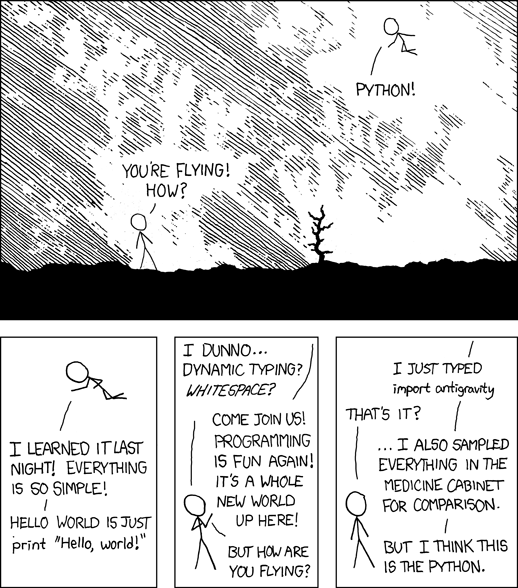
\includegraphics[width=0.6\textwidth]{reportCh2/python}
  \caption{Python by xkcd\cite{python_xkcd}}
  \label{fig:python}
\end{figure}

\subsection{Virtual Environment}
\label{virtualenv}
Virtualenv\cite{virtualenvlit} is the tool used to create isolated Python environments. Thanks to that, it is possible to make several distinct environments, which share the same version of Python, but can have different sets of modules, libraries and packages. All of them are installed in the Python \emph{site-packages} directory.

This tool is protecting applications against conflicts caused by different requirements.

\subsection{Pylons}
\label{pylons_descriptions}
Pylons \cite{pylons} is an flexible Python framework based on the MVC\footnote{MVC stands for \emph{Model-View-Controller}, more in section \ref{mvc}} design pattern and WSGI\footnote{WSGI\cite{wsgi} stands for \emph{Web Server Gateway Interface} and it is the Python standard which specifies interface between web servers and web applications.} standard. Besides base web application server functions, Pylons provides also a set of tools and libraries which extend its way of working, but it does not impose the specific solutions and tools should be used. User can decide which modules he/she wants to include in his/her application. This approach assures user that his/her application consists only of necessary modules and it is as light as possible. If it is necessary, adding third-party libraries is also very easy and intuitive. This possibility of choosing, adding and composing modules makes Pylons very flexible and light framework. It is also very easy to learn and to use by new users.

As it is written above, Pylons provides a lot of tools which simplify creating a web application. One of main ones, Routes\cite{routes} framework generates and maps URL addresses to code. Another tool, WebHelpers\cite{webhelpers} is a set of utility functions for generating JavaScript\cite{javascript} code. To create HTML code combined with Python and to pass variables to them, Pylons is using a \emph{templating system}. It allows user to write HTML and embed Python code when it is needed\cite{templating_system}. This solution also supports reusability of the code. The default templating language is Mako\cite{mako}. 

Pylons also can operate on databases (using \emph{Object Relational Managers} like in example SQLAlchemy\cite{sqlalchemy} or SQLObject\cite{sqlobject}). In addition it provides caching mechanisms and manages session variables.

\subsection{Web Application Technologies}
\label{web_application_technologies}

Interactions between users and server are handled by Ajax\cite{ajax} (Asynchronous JavaScript and XML). Due to that technology user view can be refreshed without reloading whole document. It is performed in a asynchronous way, which enables user to execute other operations at the same time. Ajax technology is built in Pylons. 


Ajax is used also by JQuery\cite{jquery}, a light and fast library that contains tools to use Javascript in more advanced way like animations or dynamic modifications of site content. What is important, changes provided by JQuery do not require modifications of HTML code of the site.

\subsection{Other tools}
\label{other_technologies}

\begin{itemize}
  \item {\bf Pygments}\cite{pygments} is a Python syntax highlighting library. It supports a significant number of languages and markup formats. There is also mechanism which allows user to define his/her own parser to recognize user specific language. Pygments can be used as a library or as a command-line tool.
  \item {\bf Pyrops} is a Python module based on {\bf pyro} - PYthon Remote Objects\cite{pyro}. Pyrops was created as a solution for the problem of concurrent accesses to Pips workspaces - it was not possible to work on several workspaces at the same time in a script\cite{pyps_doc}. Pyrops encapsulate each workspace in a new, separate program in a transparent way\footnote{Transparency is provided by RPC (and by pyro)\cite{pyps_pass_manager}}. Usage of Pyrops is easy for Pyps user - Pyrops workspace inherites of Pyps workspace and they are used in the same way.
  \item {\bf GCC}\cite{gcc} - the GNU Compiler Collection is the one of the most popular compiler for C and C++ languages. In PaWS, GCC is used for checking correctness of the user input before performing operations.
  \item {\bf F77}\cite{fortran77} and {\bf gFortran}\cite{gfortran} are Fortran compilers, which compiles Fortran code to C code. They are used in PaWS for the same reason as GCC - to check input source code.
  \item {\bf Fabric}\cite{fabric} - the Python library for automatic deployment and setting up of the application. It can be used as library but also as command-line tool. Creator of the application must provide requirements file where all of the dependencies of the application and its versions are described. A second file must be supplied. It is so called \emph{fabfile.py}. It specifies all the operations (like setup, installation, clean etc.) that can be used.
%%  \item {\bf versioning}
%%   ??
\end{itemize}




\section{Components Used}
\label{components_used}

This section provides information about specific solutions and
workarounds used in PaWS application.

\begin{itemize}

  \item {\bf Creating graphics} 
  
    Functional requirement No. \ref{req:dependence_graphs} specifies
    that PaWS must be able to create and present dependence graphs. To
    create them in \emph{dot} \cite{dot_format} format\footnote{The
      DOT language is a description language for describing graphs in
      a human and machine readable format.} a PIPS mechanism is used
    (shown in the listing \ref{DotDependenceGraphPrinting}).
  
  \lstset{language=Python,caption={Dependence graph in dot format printing},label=DotDependenceGraphPrinting}
  \begin{lstlisting}
function.print_dot_dependence_graph()
  \end{lstlisting}
  
  A file in \emph{dot} format is transformed into an image in
  \emph{png} format by command \emph{dot} of GraphViz
  Software\cite{graphviz}. Details can be found in \emph{dot} user
  manual: \url{http://www.graphviz.org/pdf/dot.1.pdf}.
  
  \item {\bf Presenting graphics} 
  
    To present dependence graphs, the jQZoom Evolution\cite{jqzoom}
    library is used. This is a light plugin based on JQuery, described
    in \ref{web_application_technologies}. It allows to present the
    image in more user-friendly way. There is small
    thumbnail\footnote{Thumbnail is the small illustration which
      represents the original image at a much smaller size.} shown and
    hoovering mouse over it enables zooming preview of selected part
    of the original, the large image. Moreover this plugin is very easy
    to use, due to its usage of JQuery, and to integrate with PaWS.
  
    The only potential problem of jQZoom usage is the need to provide
    two copies of the image in two sizes: big and thumbnail. To
    fulfill this requirement the Python Image Library (PIL) \cite{pil}
    is used. This is a Python module, which provides all the operations
    dedicated to images processing and supports many files formats. It
    is written in Python and hence is very easy to integrate in the PaWS
    framework. This is its main advantage.
  
  \item {\bf Uploading files}
  
    According to the functional requirement
    No. \ref{req:uploading_files}, PaWS enables user to browse and
    pick his/her own files. Uploading user files caused two problems:

  \begin{itemize}

  \item HTML ``input'' with \emph{type=``file''} used for uploading
    files is not customizable. That means that it is impossible to
    change the style of the button and file name label, which is
    causing aesthetic conflict with the rest of the HTML site.

  \item Uploading files through AJAX requests is impossible because of
    the browsers restrictions and the XmlHttpRequest object
    limitations\cite{ajax_files_upload}. At the same time, PaWS needs
    to be able to upload user files without refreshing the site. Since the
    stardard HTML solution is causing site refreshing, this requires
    the usage of AJAX.

  \end{itemize}
  
  The first problem is easy to solve by creating transparent files
  upload panel which covers false, styled panel (button and file name
  label). Due to that solution, only well styled button and label are
  visible but they are not active - invisible layer of not properly
  styled files upload panel captures users activity.
  
  The second problem is more serious, but it has also been solved. There
  is a hidden, also transparent and invisible, IFrame used as a target
  for file uploading (``target'' attribute is used). When a form with
  the file upload is submitted, the result will be present in a hidden,
  refreshed IFrame, but it can not be seen by user. Content of this
  frame is copied to its proper destination, the visible window. The last
  step is very easy and can be done without refreshing the whole page.
  
  \item {\bf Loading multiple files}
  
    The same requirement No. \ref{req:uploading_files} results in the
    possibility to load several user files packed in one archive file,
    using ``zip'' extension. The only restriction is that all files
    must be written in the same programming language. It is due to
    PyPS framework current limitations.
  
    Python module \emph{zipfile}\cite{zipfile} is used to handle this
    case. It provides archive creating, reading, writing and listing.
  
    For each file, a new tab is created and, when performing an
    operation, the user has to choose one specific function to
    analyse/transform. Dependence graphs are created for all functions
    from all the files.
  
  \item {\bf Printing Result Files}
  
    Functional requirement No.~\ref{req:printing_results} requests the
    possibility of printing the results of the PIPS analyses and
    transformations. To print only the results, not a whole WEB page,
    a special hidden, user invisible frame is used. At user request,
    computation result is loaded into the invisible frame which is
    printed.
  
    There is another possible solution for printing only part of a WEB
    page - usage of special style class which defines which parts of
    the site should be visible when the page is printed. The disadvantage
    of this approach is that it prints all of the page, even if a large
    part of it is invisible, which causes a large wasting of the
    space.
  
  \item {\bf Language detection}
  
    Functional requirement No. \ref{req:language_detection} refers to
    the language detection. It is based on simple tokens
    recognition. It can distinguish between C and Fortran only.
  %% In addition, distinction between different versions of Fortran language (77 and 95) needs compilation.

  %% TO ADD: mechanism! Event when typing source code, pre-compilation
  
  \item {\bf Deleting temporary files}
  
    Most temporary files created during PaWS operations are deleted
    immediately after use. Unfortunately, there are also files which
    need to be kept on the server for a longer time. This applies to
    the files which are used to present results to user, graphs images
    or files with result of transformations and analysis for
    download. To preserve disk space on the server side, requirement
    No. \ref{req:deleting_files}, a cron\footnote{It is a customizable
      Linux job scheduler, which runs periodically user scripts or
      commands\cite{cron}.} task is used. Every hour, a Python script,
    \emph{pawsd.py}, located in \emph{pawsapp$\backslash$utils}
    directory, is invoked to delete all temporary files older than 2
    hours.
  
\end{itemize}

\section{Encountered problems}
\label{encountered_problems}

PaWS implementation process encountered several problems and bugs:

\begin{itemize}
  \item {\bf Perserving consistency between output of Tpips and Pyps computations}
  
  At the beginning operations over prepared examples where performed with Tpips script, while user provided code was handled by Pyps. Also supplied example after user modification were analyze or transformed with Pyps. That was causing lack of consistency in the output - Pyps in the basic level is working with the default values, while in the Tpips script other settings can be used as well. Also style of the output performed by the Tpips and Pyps is slightly different. To provide completely consistent output all operation in the tools mode (for basic and for advanced levels) are performed by Pyps. Tpips is used in demonstration mode (which needs script with a set of well-defined operations, which is not modified by a user).
  
  \item {\bf Validation of the Pyps code}
  
  PIPS and Pyps are constantly in the development process. That can cause that the Pyps code used for the PaWS operations might require changes according to the Pyps changes. To minimize problems resulting from this, such as getting a wrong output or being unable to perform operations, all of the Pyps code used in PaWS is moved to the \emph{validation} directory, where it can undergo validation process and be easily changed if it is needed.
  
  \item {\bf Updating PIPS automatically}
  
  This problem is related to the previous one - PIPS framework, which is still changing, has to be update frequently, to let the users try the newest version of it. With automatic update, there might be a problem when current version of PIPS contains bugs or is even broken. To avoid such situation PIPS update is made manually.
  
  \item {\bf Provide concurrent access}
  
  Pylons framework creates new thread for each user request. It might cause problems with Pyps which requires new process. Pyrops (see Section \ref{other_technologies}) module, which separates Pyps workspaces, was the solution of this problem. Pyrops is also under development (it is build in Pyps).
  %% bug with sharing workspaces?
  
  \item {\bf Overloading server}
  
  Too many user requests might overload the server. Problem was not solved for the time being.
  
  \item {\bf Points to the documentation}
  
  User should have information about the PIPS properties and analyses which might be used in advanced level of tools mode. The best option to provide it is by linking them to the proper sections in the PIPS online documentation (\url{http://cri.ensmp.fr/pips/pipsmake-rc.htdoc/}). Problem is with extracting exact addresses of the sections - they are generated randomly and changing during the documentation compilation. Currently information about the PIPS settings (properties, analyses and phases) is provided by the description files.

\end{itemize}

\section{Conclusion}

Up to now, the architecture and the tools selected have met all the
requirements (see Section \ref{design_requirements}) and design
contraints (see Section \ref{design_contraints}).




\chapter{Configuration guide}
\label{configuration_guide}

This chapter is an important part for all PIPS contributors who want to configure, develop or maintain the PaWS framework. The current configuration of the project and the ways to change it, are discussed here. Also possible extensions and additions are presented in this chapter. Last sections contain the information about PaWS installation and deployment. 

\section{Current configuration}
\label{currentconfiguration}

This section contains information necessary to understand how PaWS is configured.

\subsection{Configuration file}

The initial settings for PaWS are stored in a configuration file named \emph{paws.py} in Pylons configuration directory \emph{pawsapp/config}. Parameters stored there are i.e. paths to the directories with PaWS helper files.

The configuration file is written in Python. Thanks to that it can be imported as a Python module and no parsing of the file is needed to extract settings. Parameters can also be defined as a Python variables.

\subsection{Introduction page}

The entry web page (\emph{pass/index}) contains information about all the PaWS modes and their cases. The site is hosted by template \emph{paas.mako} and controller \emph{paas.py}, but the content of the site is based on the structure of description files described below. During each site loading, information about available tools and their descriptions is loaded from that directory. The site HTML code is generated dynamically from scratch using this information.

When a new tool is added, a script added creates the description file and places it in the right place of the structure.

\subsection{Descriptions files}

Description files are placed in validation \emph{validation/Paws} directory. This directory consists of subdirectories corresponding to the particular PaWS modes and two extra description files located in \emph{validation/Paws/main} directory: \emph{paas.txt} and \emph{functionalities.txt}. 

The subdirectories contain the description files for all of the cases of the mode they are refering to. For example, the subdirectory of the {\bf tools} mode currently contains files: \emph{in\_regions.txt}, \emph{openmp.txt}, \emph{out\_regions.txt}, \emph{preconditions.txt} and \emph{regions.txt}.

The first file from \emph{main} directory, \emph{paas.txt}, provides a general description of the PaWS framework. This description is visible on the main entrance page. The second file, \emph{functionalities.txt}, gathers information about PaWS modes: their title, visible on the entry page, name of the subdirectory with case descriptions, and flag indicating whether mode has two levels, basic and advanced, or not.

\subsection{Analysis and transformations}

Currently, there are four analyses and one transformation available: \emph{preconditions}, \emph{OpenMP}, \emph{IN regions}, \emph{OUT regions} and \emph{regions}. Each of them has basic level. Two of them, \emph{preconditions} and \emph{regions} also have an advanced level configured.

As written above, descriptions of the analysis and transformation tools are placed in the \emph{validation/Paws/tools} subdirectories and examples are in the \emph{validation/Paws/$<$tool\_name$>$} directories.

The \emph{skeleton.mako} template is responsible for code of all the sites generation. There are two more specific templates inheriting from it - for basic level \emph{base.mako} and for advanced one \emph{advanced\_base.mako}. Together they provide complete support for all analyses and transformations.

Pages dedicated to a different tool, both for basic and advanced mode, are hosted by a special controller, named \emph{tools\_$<$tool\_name$>$.py} and are customized by a Mako template, named \emph{tools\_$<$tool\_name$>$.mako} or \emph{tools\_$<$tool\_name$>$\_advanced.mako} for advanced mode. Controller and templates are created automatically when a new tool is added as described in Section \ref{add_analysis_transformation}. For detailed files structure see Figure \ref{fig:paws_structure}.

\subsubsection{Advanced mode}

The advanced mode of analysis and transformations adds more user control to the base level. It is possible to choose properties which will be used when performing operation. The user is also able to select concrete kind of analysis (or transformation) that will be activated and phases to be applied before the result is displayed. 

Advanced mode examples are stored in \emph{validation/Paws/tools/$<$tool\_name$>$} directories and they are shared with the basic mode.

Content of the web pages forms for those settings selection is created dynamically. It is based on the lists of possible properties, analyses and phases. Those lists are stored in \emph{validation/Paws/tools/$<$tool\_name$>$} directories. Each of those files has its own structure:

\begin{itemize}

  \item {\bf Properties} are grouped in three categories: boolean, integer and string properties. Each property should be declared in the new line as it is shown in the Listing \ref{PropertyDeclaration}\footnote{Sign \emph{``-''} means that any value is possible.}.
  
\lstset{language=Python,caption={Property declaration},label=PropertyDeclaration}
\begin{lstlisting}
PROPERTY_NAME;default_value;value_1;other_values...;description
\end{lstlisting}

  \item {\bf Analyses} are grouped by modules. In example module \emph{preconditions} has 4 analyses (\emph{preconditions\_intra\_full}, \emph{preconditions\_inter\_fast}, \emph{preconditions\_intra\_fast}, \emph{preconditions\_intra}). In a given module, only one analysis can be selected. Analyses should be declared in the new line as it is in the Listing \ref{AnalysesDeclaration}.
  
  \lstset{language=Python,caption={Analyses declaration},label=AnalysesDeclaration}
\begin{lstlisting}
<<MODULE_NAME>>
default_analysis_name;description
analysis_1_name;description
...
\end{lstlisting}
  
  \item {\bf Phases} are also declared in new lines each. Example is shown in the Listing \ref{PhasesDeclaration}.
  
  \lstset{language=Python,caption={Phases declaration},label=PhasesDeclaration}
\begin{lstlisting}
phases_1_name;default_value;description
phases_2_name;default_value;description
...
\end{lstlisting}

\end{itemize}

\subsection{Demonstrations}

There are three demonstrations available: \emph{aile\_excerpt}, \emph{convol} and \emph{acca-2011}. Descriptions of all the cases are placed in \emph{pawsapp/public/descriptions/tutorial} directory.

Each demonstration consists in an example source code, in C or Fortran, and a Tpips script. They are found in \emph{validation/Paws/demo} directory.

Controller \emph{demo.py} and template \emph{demo.mako} are providing skeleton of the HTML code and basic functions common to all the demonstrations. As in the case of analysis and transformations, each demonstration is hosted by specific controller (named \emph{tutorial\_$<$demo\_name$>$.py}) and a Mako template (named \emph{tutorial\_$<$demo\_name$>$.mako}). The automatic creation of them is described in Section \ref{add_demonstration}.

Each Tpips script used in a demonstration is parsed and divided in several steps. Markers for separating the steps are the lines starting with the command ``display''. It is the signal that the result of the operations should be shown to the user. Not only result of the step is displayed, but also the Tpips commands of the step are presented to the user.

A second thing which is very important for those who are designing demonstration cases, is the ways comments can be inserted in the output. There are two ways to do that:

\begin{itemize}
  \item {\bf comments in Tpips script output} are simple bash comments as it is shown in the Listing \ref{TpipsComments}:
  
  \lstset{language=Python,caption={Comments in Tpips script output},label=TpipsComments}
  \begin{lstlisting}
# Remove existing workspace, if any
delete acca-2011
  \end{lstlisting}
  
  They are displayed as a part of the Tpips script linked to the current step.
  
  \item {\bf comments in result output} are created by writing message to standard output with \emph{echo}\cite{echo} bash\cite{bash} command. It is important to remember that comments should be suitable with the relevant programming language comments style. Example of creating comments for C output is shown in Listing \ref{EchoComments}:
    
  \lstset{language=bash,caption={Comments in step result output},label=EchoComments}
  \begin{lstlisting}
echo '/*'
echo ' * Source code for "compute" function.'
echo ' */'
echo
  \end{lstlisting}
  
  These comments are displayed in the output window.
  
\end{itemize}

\subsection{Examples}

All examples for all of analysis and transformations are stored in the validation directory \emph{validation/Paws}. Adding new example is very easy and the process is described in the Section \ref{add_example}.

There is special controller \emph{examples.py} designed to handle the examples. It is responsible for getting information about available examples and for loading file contents.

\subsection{Python code}

Python code is located in the \emph{validation/Paws/pyps\_modules} directory. File \emph{paws\_base.py} is responsible for the basic operation, such as opening and closing the workspace or setting properties. Each analysis or transformation has its own file with \emph{invoke\_function} method which is responsible for concreate operation, i.e. for preconditions, file \emph{paws\_preconditions.py} contains code for getting preconditions code.

\section{How to Configure PaWS}

Extending the PaWS framework is very easy and intuitive. In all cases
it is sufficient to create a new directory, add a description file or
invoke a simple script. All the details are described in this section.

\subsection{How to Add a New Analysis or Transformation}
\label{add_analysis_transformation}

Adding a new pass, a PIPS analysis or transformation, is handled by a
script, which simplifies the whole process. It is possible, thanks to
the generic approach and the supplied templates, to create dynamically
each WEB page.

The Shell script \emph{add\_tool} creates all necessary files for both modes,
such as controller, basic and advanced mako templates, skeleton of the
file with PyPS code, described below, and validation subdirectory with the
description file and empty lists with properties, analyses and phases
for advanced mode. These must be filled in by the configurer.

The configurer needs to provide four of five arguments to the script:

\begin{itemize}

  \item {\bf the name of the tool} which will be used as ID of the operation;

  \item {\bf the header of the page} which will be displayed at the
    top of the web page; if it is longer than one word, it should be
    surrounded by parentheses;

  \item {\bf the description of the tool} which will be placed in the
    description file and visible on the introduction page; if it is
    longer than one word, it should be surrounded by parentheses;

  \item {\bf PyPS print code module} to print the code of the
    operation. Script will create sample code in the directory of PyPS
    modules (\emph{validation/Paws/pyps\_modules}) and test for
    validation. If the code should be different than default, shown in
    Listing~\ref{DefaultPyps}, it has to be updated manually;

  \item {\bf the directory containing the existing examples} -
    optional. They will be copied into the validation directory
    (\emph{validation/Paws/tools/$<$operation\_id$>$}); if this
    argument is not provided, directory
    \emph{validation/Paws/tools/$<$operation\_id$>$} is created but it
    remains empty.
  
\lstset{language=Python,caption={Default PyPS Code},label=DefaultPyps}
\begin{lstlisting}
def invoke_function(function, workspace):
	return function._get_code(activate = module.<print_code_module>)
\end{lstlisting}
  
\end{itemize}

The Shell script \emph{add\_tool} is placed in
\emph{paws\_app$\backslash$utils} directory. It is a bash script. See
Listing~\ref{AddToolUsage} for an invocation example.

\lstset{language=bash,caption={Usage of \emph{add\_tool} script},label=AddToolUsage}
  \begin{lstlisting}
. add_tool <name> <header> <description> <examples_dir> <pyps_module>
  \end{lstlisting}

\subsection{How to Add a New Demonstration}
\label{add_demonstration}

The addition of a new demonstration is also handled by a Shell script. The
user needs to provide only two arguments:

\begin{itemize}

\item {\bf the source file} is the example file on which the TPIPS
  script, which should have the same base name and be placed in the same
  directory, will perform operations;

\item {\bf a description of the case} which will be placed in the
  description file and visible on the introduction page; if it is
  longer than one word, it should be surrounded by parentheses.

\end{itemize}

The script \emph{add\_demo} is placed in direcotry
\emph{paws\_app$\backslash$utils}. It is a bash script. The
Listing~\ref{AddDemoUsage} provides an invocation example.

\lstset{language=bash,caption={Usage of \emph{add\_demo} script},label=AddDemoUsage}
  \begin{lstlisting}
. add_demo <source_file> <description>
  \end{lstlisting}

\subsection{How to Add a New Example}
\label{add_example}

Adding new example for an existing tool is very easy. It is sufficient
to place the new example file in the adequate subdirectory of the
tools validation directory,
\emph{validation/Paws/tools}. Subdirectories are described in the
Section~\ref{other_modules}. Added example will be automatically
visible on the WEB page of the tool it refers to when the user browses
the tool examples.



\section{PaWS deployment and managing}
\label{paws_managing}

PaWS is based on Pylons \cite{pylons} framework which is WSGI\footnote{WSGI stands for \emph{Web Server Gateway Interface} \cite{wsgi} - Python specification for web servers, applications and web applications for communication standardization.} compliant. This standard provides a lot of ways to deploy the web applications, depending on their needs \cite{python_app_deployment}.

The easiest way is based on \emph{Paste Script} module \cite{paster}, which is part of the Pylons and provides necessary server commands, such as:

\begin{itemize}
  \item {\bf Start the server}
  
\lstset{language=Python,caption={Starting the server},label=StartServer}
\begin{lstlisting}
. utils/pipsenv.sh
paster serve --reload development.ini
\end{lstlisting}
  
  \item {\bf Get status of the server}
  
\lstset{language=Python,caption={Status},label=PasterStatus}
\begin{lstlisting}
paster serve --status development.ini
\end{lstlisting}
  
  \item {\bf Create the new controller}
  
\lstset{language=Python,caption={Create the new controller},label=PasterController}
\begin{lstlisting}
paster controller <controller_name>
\end{lstlisting}
  
\end{itemize}

All those commands have to be invoked in the directory, which contains \emph{development.ini} file (see Section \ref{structure} for detailed information).

\subsection{Supervisor}

Currently PaWS server is run using Supervisor \cite{supervisor}, the system for process control and monitoring. It provides mechanism of automatic restart of the process if it crushes.

\section{Installation}
\label{installation}

Installation process is described in \emph{README.txt} file in \emph{pawsapp} directory.

%% \begin{itemize}
%%   \item For user with PIPS
%%   \item For developer with VirtualEnv
%% \end{itemize}

\section{Conclusion}

The PaWS framework was designed to be fully configurable by anybody with a good knowledge of PIPS. It does not require any knowledge of the technology used to develop PaWS.



\chapter{User Manual}

This chapter contains information and tips for users about the proper
usage of the PaWS Framework.

Should it be also available on-line?

\section{PaWS}

The introduction page presents overall information about PaWS and PIPS in the panel on the left side, as it is shown in the Figure \ref{fig:intro_page}.

\begin{figure}[h!]
  \centering
  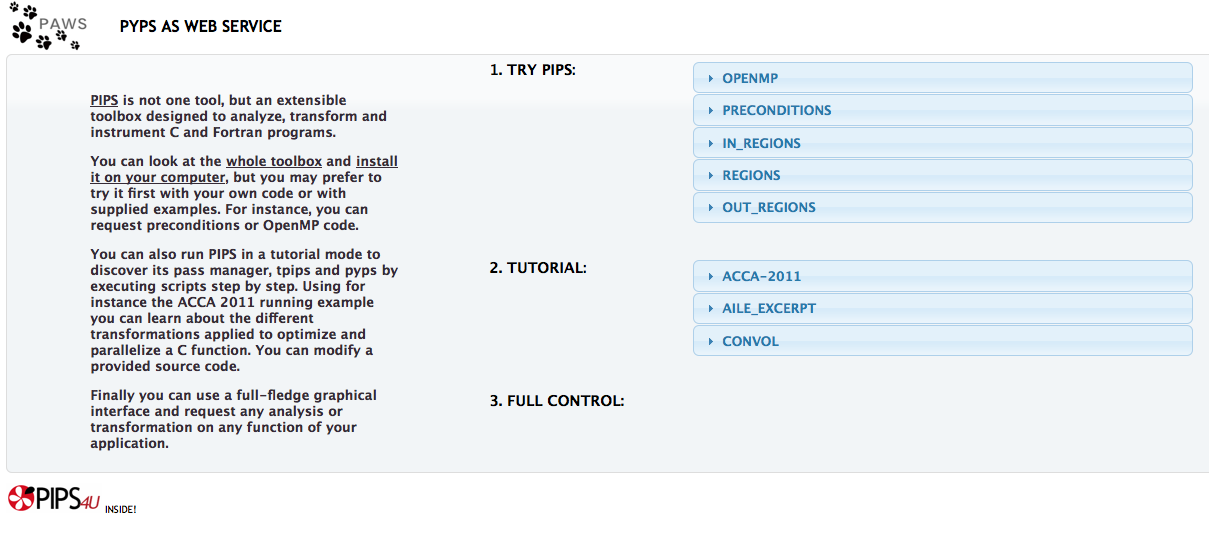
\includegraphics[width=0.8\textwidth]{reportCh4/intro_page}
  \caption{PaWS Introduction page.}
  \label{fig:intro_page}
\end{figure}

Left side panel allows the user to choose mode and its concrete tool or demonstration. To do it, the user has to click on the tab of the chosen tool/demonstration. It will be expanded (see Figure \ref{fig:expanded_tab}) with more detailed information and links to the actual sites visible.

\begin{figure}[h!]
  \centering
  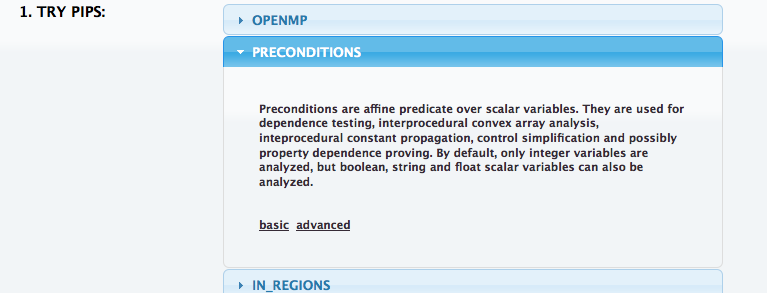
\includegraphics[width=1.0\textwidth]{reportCh4/expanded_tab}
  \caption{Expanded preconditions tab.}
  \label{fig:expanded_tab}
\end{figure}

To come back to the introduction page, the user can use logo image (see Figure \ref{fig:logo_image}) as a link.

\begin{figure}[h!]
  \centering
  
\includegraphics[width=0.2\textwidth]{reportCh4/logo_image}
  \caption{Logo image as home page link.}
  \label{fig:logo_image}
\end{figure}

\section{Basic Tools}

The basic tool provides PIPS analysis or transformation passes. They
are available in at most two levels: basic and advanced (see
Section~\ref{paws_project}).

\subsection{Basic Level}

The basic level allows the user to try PIPS analysis or transformation
with a default setting. An example page is shown in
Figure~\ref{fig:basic_mode_screen}.

\begin{figure}[h!]
  \centering
  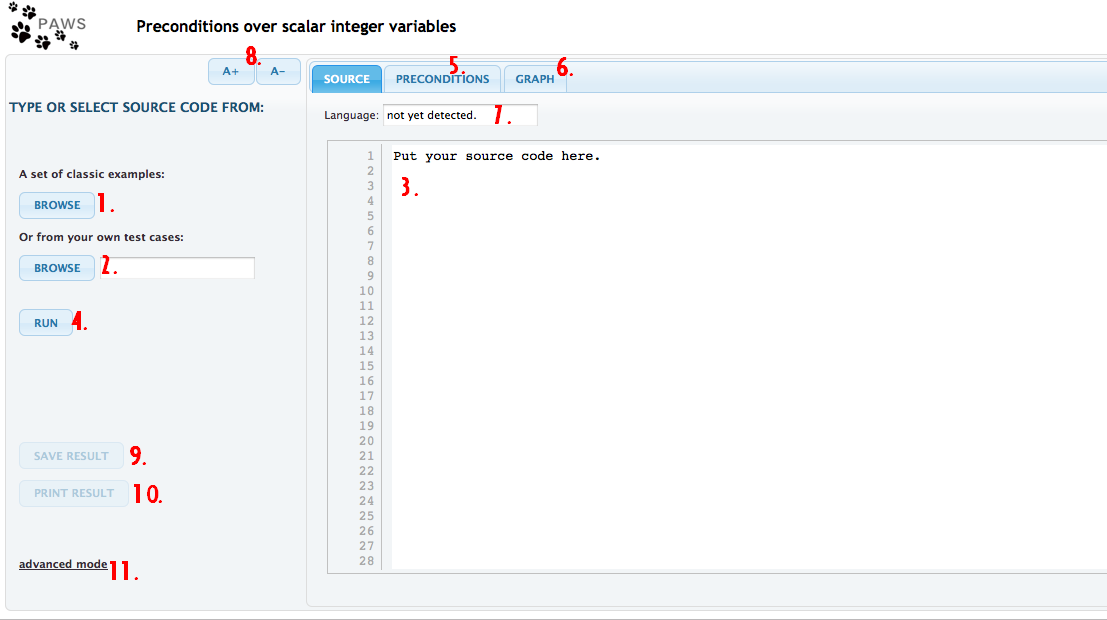
\includegraphics[width=0.8\textwidth]{reportCh4/basic_mode_screen}
  \caption{Preconditions basic level screen.}
  \label{fig:basic_mode_screen}
\end{figure}

The user can provide the source code either by loading one of supplied
examples ({\bf 1.}) or by picking it locally from his/her machine
({\bf 2.})  or by typing it in the source code window ({\bf 3.}). The
pass is launched by clicking either the button ``RUN'' ({\bf 4.}) or the
tab ``PRECONDITIONS'' ({\bf 5.}). Selecting the tab ``GRAPH'' ({\bf
  6.}) invokes the dependence graph computation and display.

After loading the source code, the language of the code is detected and
displayed in the programming language label ({\bf 7.}). In case of
inconvenience, the user can change font size used on the side by the
``A+'' and ``A-'' buttons ({\bf 8.}).

The user can save or print the results of the performed
pass. Buttons, which enable that ({\bf 9.} and {\bf 10.}),
disactivated at the beginning, are activated when the result is ready.

The link at the bottom of the page ({\bf 11.}) leads to the advanced
level mode of the same tool.

\subsection{Advanced Level}

The layout and usage of the advanced level page is very similar to the
basic one. The only difference is the possibility of setting
properties, analyses and phases (see
Figure~\ref{fig:advanced_properties}). Each setting has its
description, which is made visible when hovering the mouse over its
check button.

Boolean properties ({\bf 1.}) are set to {\bf True} or {\bf False} by
simple being checked. Integer properties ({\bf 2.}) are checked by a
default and their values can be changed by the user. After invocation
of the operation they are validated. String properties ({\bf 3.}),
analyses ({\bf 4.}) and phases ({\bf 5.}) have predefined lists of
possible values. The default one is already selected.

\begin{figure}[h!]
  \centering
  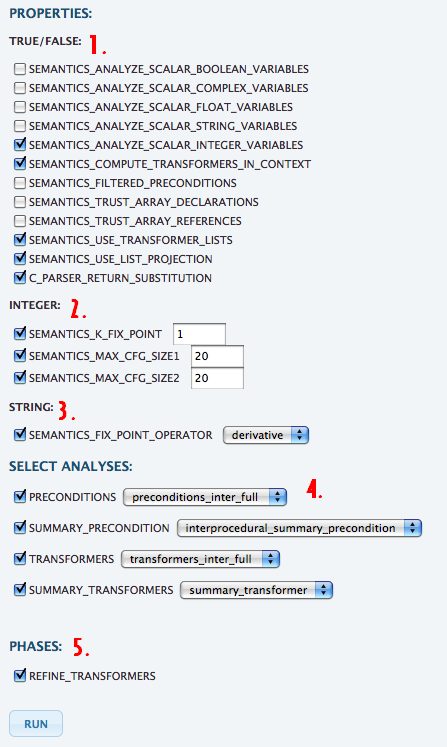
\includegraphics[width=0.5\textwidth]{reportCh4/advanced_properties}
  \caption{Forms for setting properties, analyses and phases.}
  \label{fig:advanced_properties}
\end{figure}


\section{Tutorial}

The aim of the tutorial mode is to show the user the variety of PIPS
abilities. At the begining, the chosen example is loaded, as is shown
in Figure~\ref{fig:tutorial_screen} (example ``Acca-2011'').

\begin{figure}[h!]
  \centering
  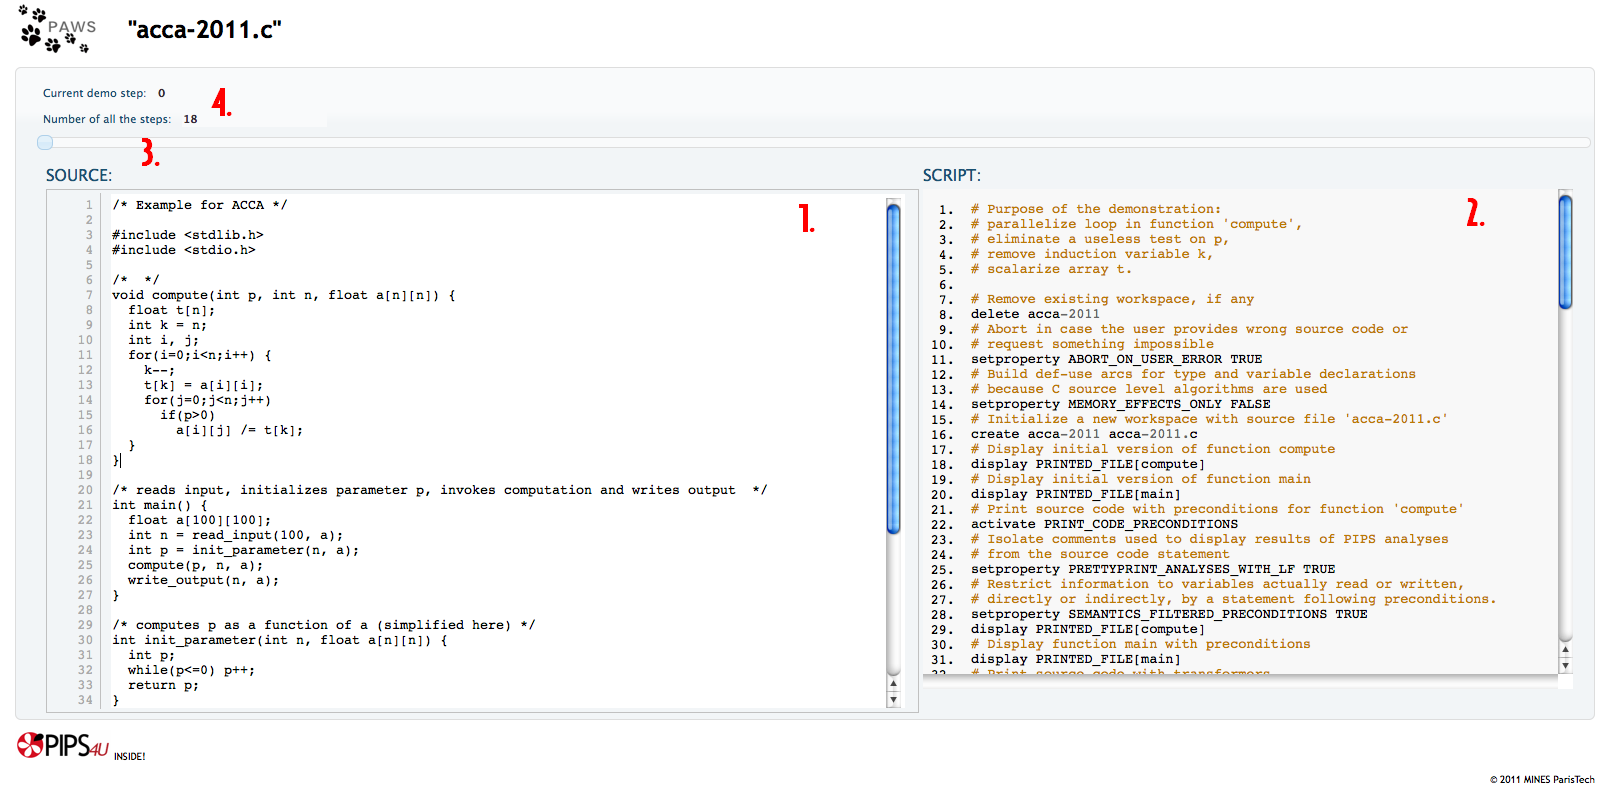
\includegraphics[width=0.8\textwidth]{reportCh4/tutorial_screen}
  \caption{``Acca-2011'' tutorial screen.}
  \label{fig:tutorial_screen}
\end{figure}

This mode does not require a significant interaction with the user -
the source code ({\bf 1.}) and the script with operations and comments
({\bf 2.}) are provided. The user only needs to change the current
step using the slider ({\bf 3.}). It is very flexible and stepping
does not have to be sequential: the user can go back or skip some
steps. The current step and the numbers of all steps are displayed
over the slider ({\bf 4.}).




The major aim of the project was to create lightweight web application, which allows to use PIPS without installing it. Other goals were to provide different types of ways of using PIPS, which were depending on user's level of advance. Whole list of constraints and functional requirements can be found in the Sections \ref{design_contraints} and \ref{design_requirements}.

To achieve those goals, web application was developed, which presents PIPS in two modes, described in the Section \ref{paws_project}. Content of all the pages of those modes is generated dynamically and is based on the structure of the directories and files with descriptions. Thanks to this solution, configuration of the PaWS is very easy and does not require knowledge of the Pylons framework.

Implemented functionality contains also a lot of user-friendly features (see requirements in the Section \ref{design_requirements} and components used \ref{components_used}), like creating, displaying and zooming graphs, resizing font size (according to user preferences), uploading user files (also archive .zip files), saving results of the operations on user's machine or printing them.

Main goal for the future is to implement third mode, full control, which will enable user to graphically create his/her own PIPS script. PaWS should also have more tests - currently there are no tests for its graphical interface. Other new utility would be Pyps/Tpips code generation with all the properties, analyses and phases used (for advanced mode). Also possibility of saving and printing dependence graphs would be useful.

Other small, possible improvements are:
\begin{itemize}
  \item Adding the scale for a slider in demonstation module.
  \item Control the time of the response from the server.
  \item Integration of the IR Navigator \cite{irnavigator}.
\end{itemize}

Current version of the PaWS framework meets all the design constraints and requirements imposed at the beginning. It can also be easily extended with the new functionality.

%%\begin{ilustracje}
%%\listoffigures
%%\end{ilustracje}

%%\begin{listingi}

%%\end{listingi}

%%\begin{skroty}

%%\end{skroty}





%% ======== BIBLIOGRAFIA ========
%%
%% ************ AKADEMIA G/ORNICZO-HUTNICZA W KRAKOWIE *************
%% ***************** Wydzial Matematyki Stosowanej *****************
%% ****************** PRACA MAGISTERSKA w LaTeX-u ******************
%%    autor: ------
%%    Copyright (C) 2002 by ------
%% ******************** Plik z literatura *************************
%%

% \bibliography{reportRoot}

\begin{thebibliography}{88}
\normalsize
\addtolength{\itemsep}{\smallskipamount} % tak dla przejrzystosci

\bibitem{wir2011} Fabien Coelho, Pierre Jouvelot, Corinne Ancourt, Francois Irigoin: \textit{Data and Process Abstraction in PIPS Internal Representation}, Chamonix, 2011

\bibitem{ics1991} Francois Irigoin, Pierre Jouvelot, Remi Triolet: \textit{Semantical Interprocedural Parallelization: an Overview of the PIPS Project}, Cologne, 1991

\bibitem{pyps_pass_manager} Serge Guelton, Gregoire Payen de La Garanderie: \textit{Pyps Pass Manager}, Telecom Bretagne, 2010

\bibitem{pyps_doc} Gregoire Payen de La Garanderie: \textit{A tutorial for Pyps}, Telecom Bretagne, 2010

\bibitem{service_def} Krzysztof Zielinski: Service Oriented Architecture. AGH University of Science and Technology, Krakow

%%\bibitem{thomas_erl} Erl T.: \textit{SOA Principles of Service Design}. Prentice Hall, 2007. 

%%\bibitem{don_box} Box D.: \textit{Essential COM}. Addison-Wesley Longman, 1998.


%% linki i website'y: alfabetycznie

\ \\ 

{\large \textbf{Internet sources}}\\* 

\bibitem{cri} CRI
\url{http://cri.ensmp.fr}

\bibitem{pips4u} PIPS framework
\url{http://pips4u.org}

\bibitem{pips_make} PIPS technical documentation
\url{http://www.cri.ensmp.fr/pips/pipsmake-rc.htdoc}

\bibitem{pylons} Pylons Project
\url{http://pylonsproject.org}

\bibitem{pygments} Pygments - Python syntax highlighter
\url{http://pygments.org}

\bibitem{fabric} Fabric
\url{http://docs.fabfile.org/en/1.0.1/index.html}

\bibitem{gcc} the GNU Compiler Collection
\url{http://gcc.gnu.org}

\bibitem{fortran77} GNU Fortran 77
\url{http://www.kilmnj.com/g77}

\bibitem{gfortran} gfortran - the GNU Fortran compiler
\url{http://gcc.gnu.org/wiki/GFortran}

\bibitem{mvc} Model-View-Controller design pattern
\url{http://www.enode.com/x/markup/tutorial/mvc.html}

\bibitem{wsgi} WSGI tutorial
\url{http://webpython.codepoint.net/wsgi_tutorial}

\bibitem{sqlalchemy} SQLAlchemy
\url{http://www.sqlalchemy.org}

\bibitem{sqlobject} SQLObject
\url{http://sqlobject.org}

\bibitem{mako} Mako Template
\url{http://www.makotemplates.org}

\bibitem{webhelpers} WebHelpers
\url{http://sluggo.scrapping.cc/python/WebHelpers/index.html}

\bibitem{routes} Routes
\url{http://routes.groovie.org}

\bibitem{ajax} Ajax
\url{http://www.xul.fr/en-xml-ajax.html}

\bibitem{javascript} JavaScript Introduction
\url{http://www.w3schools.com/js/js_intro.asp}

\bibitem{jquery} JQuery
\url{http://jquery.com}

\bibitem{python_xkcd} Python by xkcd
\url{http://xkcd.com/353}

\bibitem{templating_system} Using View Templates
\url{http://pylonsbook.com/en/1.1/using-view-templates.html}

\bibitem{pyro} PYthon Remote Objects
\url{http://irmen.home.xs4all.nl/pyro3}

\bibitem{mvc_for_php} MVC for Php
\url{http://www.tonymarston.net/php-mysql/model-view-controller.html}

\bibitem{echo} Echo command
\url{http://www.linfo.org/echo.html}

\bibitem{bash} Bash GNU Project
\url{http://www.gnu.org/software/bash}

\bibitem{virtualenvlit} Virtual Environment
\url{http://pypi.python.org/pypi/virtualenv}

\bibitem{jqzoom} jQZoom Evolution
\url{http://www.mind-projects.it/jqzoom_v10}

\bibitem{pil} Python Image Library
\url{http://www.pythonware.com/products/pil}

\bibitem{dot_format} The DOT language
\url{http://www.graphviz.org/doc/info/lang.html}

\bibitem{graphviz} Graphviz - Graph Visualization Software
\url{http://www.graphviz.org}

\bibitem{ajax_files_upload} AJAX and File Upload
\url{http://www.telerik.com/help/aspnet/ajax/ajxajaxandupload.html}

\bibitem{cgi} Common Gateway Interface
\url{http://www.w3.org/CGI}

\bibitem{cheetah} Cheetah - The Python-Powered Template Engine
\url{http://www.cheetahtemplate.org}

\bibitem{jinja2} Jinja2 (The Python Template Engine)
\url{http://jinja.pocoo.org}

\bibitem{django} Django Project
\url{https://www.djangoproject.com}

\bibitem{turbogears} TurboGears Web Framework
\url{http://turbogears.org}

\bibitem{rubyonrails} Ruby on Rails
\url{www.rubyonrails.org}

\bibitem{symfony} Symfony - Web PHP Framework
\url{http://www.symfony-project.org}

\bibitem{cakephp} CakePHP: the rapid development php framework
\url{cakephp.org}

\bibitem{yii} Yii PHP Framework
\url{www.yiiframework.com}

\bibitem{orm} Mapping Objects to Relational Databases: O/R Mapping In Detail
\url{http://www.agiledata.org/essays/mappingObjects.html}

\bibitem{cron} Introduction to cron
\url{http://www.unixgeeks.org/security/newbie/unix/cron-1.html}

\bibitem{zipfile} Zipfile module
\url{http://docs.python.org/library/zipfile.html}

\bibitem{cherrypy} CherryPy
\url{http://www.cherrypy.org}

\bibitem{paster} Python Paste
\url{http://pythonpaste.org}

\bibitem{supervisor} Supervisor: A Process Control System
\url{http://supervisord.org/index.html}

\bibitem{wsgi} Web Server Gateway Interface
\url{http://wsgi.org/wsgi}

\bibitem{python_app_deployment} Python web application deployment
\url{http://pylonsbook.com/en/1.1/deployment.html}

\bibitem{ws_standard} Web Service standard
\url{http://www.w3.org/2002/ws}

\bibitem{agilemethodology} Agile Methodology
\url{http://agilemethodology.org}

\bibitem{irnavigator} IR Navigator
\url{http://pips4u.org/doc/ir-navigator}

\end{thebibliography}
%%
%% ======== DODATKOWE ELEMENTY (nieobowiązkowe) ======== 
%%
%\printindex  
%%

\end{document}

